\chapter{Prior works leading to \posl}
\label{chap:prior}
%\textit{In this chapter are presented Prior works leading to \af. In Section~\ref{sec:relaxation} we explain how to tackle \csps{} by modeling it through a continuous optimization problem, as a first attempt aiming for the right direction in order to find the proper approach. In Section~\ref{sec:split} we present a brief work where we applied the the {\it problem subdivision} approach to solve the {\it k-medoids problem} in parallel. Finally we present in Section~\ref{sec:paramils} a study applying the {\sc ParamILS} tool in order to find the optimum parameter configuration to {\it Adaptive Search} solver.}
\textit{In this chapter are presented Prior works leading to \posl. In Section~\ref{sec:split} we present a brief work where we applied the {\it problem subdivision} approach to solve the {\it k-medoids problem} in parallel, as a first attempt aiming for the right direction in order to find the proper approach. Finally we present in Section~\ref{sec:paramils} a study applying the {\sc ParamILS} tool in order to find the optimum parameter configuration to {\it Adaptive Search} solver.}

\vspace{2ex}\vfill
\minitoc
\newpage

%\section{Relaxation model for discrete \csps}
%\label{sec:relaxation}

%Aiming for the right direction in order to find the proper approach, our first attempt to tackle the problem of reducing the search space of a \csp, we model it through a continuous optimization problem, and then, applying efficient methods to solve it. This way we do not reach an optimal solution, but an approximation of it. The new variables domain would be the neighborhood of the found approximation.

%On a first attempt to tackle the problem of reducing the search space of a CSP, we thought to model it through a continuous problem, and after, trying to apply efficient methods to solve this kind of problems. This way we do not reach an optimal solution, but an approximation of it. The new variables domain would be the neighborhood of the found approximation. In \cite{Pardalos2006} some issues to take into account in order to model combinatorial problems using continuous problems are showed.

To illustrate the fallowed procedure, we will use a widely known problem: \textit{n-queens problem}.

In the \textit{n-queens problem}, you want to place $n$ queens on an $n \times n$ chessboard (square grid). Each queen occupies one square on a grid and no two queens share the same square. Two queens are attacking each other if one of them can  travel horizontally, vertically, or diagonally and hit the square the other queen is on. The problem is to place the queens such that no two queens are attacking each other.

The Constraint Satisfaction Problem associated to the $n\times n$ N-Queens problem:

\begin{equation}
\begin{array}{rl}
\label{CSP}\text{CSP} = &\left\{\mathbb{X}, \mathbb{D(X)}, \mathbb{C}\right\}\\
\mathbb{X} =& \left(x_1, x_2, \dots, x_n\right)\\
\mathbb{D(X)} =& \left\{\mathbb{D}(x_i)\right\}, \mathbb{D}(x_i) = \left\{1, 2, \dots, n\right\}, \forall i = 1 \dots n\\
\mathbb{C} =& \left\{\mathbb{C}_1, \mathbb{C}_2\right\}
\end{array}
\end{equation}

In Model \ref{CSP}, the value of $x_i$ represent the position of a queen in the column $i$. This representation ensures that only one queen will be placed in a given column. To ensure that only one queen can be placed in a row, we can write the following constraint:

\begin{align*}
\mathbb{C}_1 &\equiv x_i \neq x_j\\
\mathbb{C}_1 &\equiv x_i - x_j > 0 \text{  or  } x_i - x_j < 0\\
\mathbb{C}_1 &\equiv \left(x_i - x_j\right)^2 > 0\text{, }\forall i < j\\
\end{align*}

Then, we only have to ensure that two queens can not be connected diagonally:

\begin{align*}
\mathbb{C}_2 &\equiv \left|x_i - x_j\right| \neq \left|j - i\right|\\
\mathbb{C}_2 &\equiv \left(x_i - x_j\right)^2 \neq \left(j - i\right)^2\\
\mathbb{C}_2 &\equiv \left(x_i - x_j \right)^2 - (j - i)^2 > 0 \text{  or  } \left(x_i - x_j\right)^2 - (j - i)^2 < 0\\
\mathbb{C}_2 &\equiv \left(\left(x_i - x_j \right)^2 - (j - i)^2\right)^2 > 0\text{, }\forall i < j\\
\end{align*}

We describe below the transformation into a non-linear optimization problem penalized.

\begin{equation}
\text{NLOP } = \left\{
\begin{array}{rrl}
\min & f(X) = & -P_1\cdot\sum\limits_{i < j}{\left(x_i - x_j\right)^2}\\
 & & - P_2\sum\limits_{i < j}{\left(\left(x_i - x_j \right)^2 - (j - i)^2\right)^2}-\\
 & & - P_3\sum\limits_{i < j}{\left(\left(x_j - x_i \right)^2 - (j - i)^2\right)^2}\\
 & X = & (x_i)\text{, } i = 1\dots n \text{ and } i < j\\
\text{s.t.: } & 1 \leq x_i \leq n & 
\end{array}
\right.
\end{equation}

The global minimum $\zeta$ exists and $f(\zeta) = 0$. The main key here is to choose $P_i\text{, }i=1..3$ big enough. In this way we obtained a non-linear optimization model with box-constraints, and from \cite{Zhu1994, Byrd1994, Liu1989} we have an efficient program to solve this kind of problems (\textit{L-BFGS-B}), even for large instances \cite{Nocedal1996}. This work provide an open source code in C\#, and to use it we had to implement a subroutine (method) called \textbf{fungrad}, telling to the algorithm how to evaluate the objective function and his gradient.

This approach did not show good results. One possible reason is that, as we can see, a quadratic model at first became in a more complex model with 4-exponent. It is fear to remark also that this problem can have several local optimums ($\bigtriangledown F(X^*) = 0$) different than the global optimum, and this algorithm returns them as solutions. In a continuous point of view two different variables have different values even when they are too close, and this can be the other reason. The previous model can be improved in order to obtain better results. Also a good idea is to choose others benchmark problems as case of study, but we decide to not keep working on that because the investigation in this field will take us further apart from the thesis main goal.

\section{Domain Split}
\label{sec:split}

%A way to tackle huge combinatorial problems in parallel is to split the search space. In this section, the {\it problem subdivision} approach was adopted to divide the domain of a given problem, in this particular case, to solve the {\it k-medoids problem} in parallel. \footnote{This work falls within the framework of the \textit{Ulysses} project between France and Ireland}

% At the very end of this section 5.1.2, by one small sentence like:
% This work falls within the framework of the Ulysse project between France and Ireland.

Usually, to solve some problem using parallelism, our first thought is either partitioning the problem into a set of sub-problems, or dividing its search space. In both cases, the idea is to solve a set of problems, all of them smaller and easer than the original one, and combining all the solution to obtain the solution of the original problem. In \cite{Arbelaez2012} a study of the impact of space-partitioning techniques on the performance of parallel local search algorithms to tackle the \textit{k-medoids} clustering problem is presented. The authors use a parallel local search, in order to improve the scalability of the sequential algorithm, which is measured, in terms of the quality of the solution, with respect to the sequential algorithm. In this work two main techniques for domain partitioning are presented: {\it space-filling curves}, used to reduce any n-dimensional representation into a one-dimension space; and {\it k-Means} algorithm. We found that the used methods for domain partitioning do not take into account the number of clients associated to each new sub-domain. This results in an unbalanced distributions of workload phenomenon. For that reason the goal of this study was designing some ideas to tackle the same problem. \footnote{This work falls within the framework of the Ulysses project between France and Ireland.}

The \textit{k-medoids} problem aims to select a subset $M$ of $k$ points (the medoids) from a set of points $S$, such that the average distance from any point to its closest medoid is minimized. It finds a lot of applications in the industry, like in resource allocation, data mining, among others. It is quite similar to \textit{k-means} problem, except that the set of medoids $M$ is forced to be a subset of $S$.

We propose Algorithm~\ref{algo}, which represents the backbone of our idea. This algorithm takes a set of $\mathbb{R}^2$ {\it points} (representing the locations of the clients) and returns a partition of size $K$. Such a set of points is called a {\it domain} and the partition a {\it sub-domain}. At each intermediate step $i$, we have a set (list) of sub-domains. The algorithm takes the most populated one, splits it into two (or four, depending on the strategy) new sub-domains and includes them in the list. The stop condition will depends on the fallowed approach (see below).

\incmargin{1.4em}
\linesnumbered
\begin{algorithm}[H]
\dontprintsemicolon
\SetLine
\SetKwData{A}{A}
\SetKwData{Q}{Q}
\SetKwData{Uni}{U}
\SetKwData{subsets}{$\left[a_1, a_2\right]$}
\SetKwData{suba}{$a_1$}
\SetKwData{subb}{$a_2$}
\SetKwFunction{GetNext}{GetNext}
\SetKwFunction{Split}{Split}
\SetKwFunction{Insert}{Insert}
\SetKwInOut{Input}{input}
\SetKwInOut{Output}{output}

\Input{\Uni : Set of client locations}
\Output{\Q = $\left\{Q_i\right\}_{i=1\dots K}$: $K$ subsets of \Uni}
\BlankLine

\A $\leftarrow$ \Uni\;
\Q .\Insert{\A}\;
\Repeat{$<$some condition$>$}{ \nllabel{paso_condicion} 
	\A $\leftarrow$ \Q .\GetNext{} \label{paso2} \tcc{It also removes the returned element}
    \subsets $\leftarrow$ \Split{\A} \label{paso3}\;
    \Q .\Insert{\suba , \subb} \label{paso4}\;
}
\caption{Domain\_Split}
\label{algo}
\end{algorithm}

First of all, we make clear some details of the algorithm exposed above:

\begin{itemize}
\item \texttt{Insert($\dots$)} Inserts a set (or two) into the data structure. % \footnote{The design was decided, because first we need to know some implementations details about the tool already coded by the Ireland team}.
\item \texttt{GetNext()} Returns the next sub-set to be divided, tacking into account the {\it split strategy} (see below).
\item \texttt{Split($\dots$)} Returns two sub-domains as a subdivision of the given domain (parameter).
\end{itemize}

In the next sub-sections we answer two main question arising at this point:

\begin{enumerate}
\item \textit{How to split the each sub-domain?} ($<$\emph{Split}$>$ function on line \ref{paso3}) It refers to, given a set of points (locations), how to decide which of them will be included into one sub-domain and which of them into the other.
\item \textit{How much to split each sub-domain?} ($<$\emph{some condition}$>$ on line \ref{paso_condicion}) It refers to decide when to stop splitting the domain.
\end{enumerate}

\subsection{Domain Splitting. General point of view}

In order to split the domain, we can think in some approaches, taking into account the number of available cores and the number of metro-nodes we want to place in the system. In the article of A.~Arbelaez and L.~Quesada a domain split taking into account the number of available cores for parallel calculus is proposed. In our approach we intend to extend this idea keeping in mind also the number of metro-nodes to allocate. Following, we propose three variants to face the problem:

% itemize variants, give the main idea in 1 or 2 paragraphs for each variant.

\begin{enumerate}
\item {\bf one metro-node per core}: In this variant we can assign one metro-node to each core, and in this case, splitting the domain in $K$ sub-domains ($K$ is the number of cores). It means that the algorithm will compute the best position for a metro-node in a current sub-domain. \label{var1}
\begin{itemize}
\item In this case we only have to replace the line \ref{paso_condicion} by something like:  \textcolor{gray}{{\bf for} $i \leftarrow 1$ {\bf to} $N$ {\bf do} $\dots$}, 
where $N$ is the number of metro-nodes.
\item The ideal scenario here is when $N = K$ which is not probable at all. So we only should study the case when they are different
\item In that case, we need to distribute efficiently the metro-nodes into the domain subdivisions, but here, one possible scenario arise: it can be happen that, depending on the followed domain-split strategy, we were trying to allocate a metro-node into an area with a few clients. This produce a very local point of view of the problem. That is the reason why we propose the following \textit{second variant}.
\end{itemize}
\item {\bf Incomplete partition}: To split a sub-domain if it can generate sub-sub-domains containing at least $C$ clients. It means, for example, if there exist in list a sub-domain with 8 clients, and the number $C$ is fixed in $C = 5$, this sub-domain can not be divided, because it will generate for sure a sub-sub-domain with less that 5 clients. In this case more than one metro-node would be allocated in some of those specific sub-domains, because we will have more metro-nodes than sub-domains in our model.\label{var2}
\begin{itemize}
\item Of course, using this variant we can find situations described in the first variant. In that case we should proceed consequently.
\end{itemize}
\item {\bf Combination}: This variant is just a combination of the two previous variants. Then, we will be working with two parameters: \label{var3}
\begin{itemize}
\item $C \rightarrow$ Lower bound of clients for new sub-domains. It means that a sub-domain can be divided iff the new produced sub-domains will contains more than $C$ clients.
\item $M \rightarrow$ Lower bound of metro-nodes to be allocated in a sub-domain. In this case we will split the domain while it can be ensure that at least $M$ metro-nodes will be assigned to each sub-domain.
\end{itemize}
\end{enumerate}

% itemize split startegies, give the main idea in 1 or 2 paragraphs for each.

\subsection{Split strategies}

In this sub-section we first discuss three ideas to split the domain. They take a sub-domain and produce other two, dividing the space vertically or horizontally, depending on the shape of the current sub--domain. In other section we expose another strategy to follow, in which the subdivision of a sub-domain produces four sub-domains.

In all of them the number of clients in each sub-domain is taken into account, but in different ways. A common feature between them is that, at the moment of splitting a given sub-domain, it will be done in a perpendicular way (either to the x--axis or to the y--axis, depending on the characteristic of the sub-domain to be divided). The reference point to divide the sub-domain is called the {\it cut point} of the sub-domain.

\begin{figure}
	\centering
	\subfloat[][Geometrical Split]{%
		\label{norm:geom}
		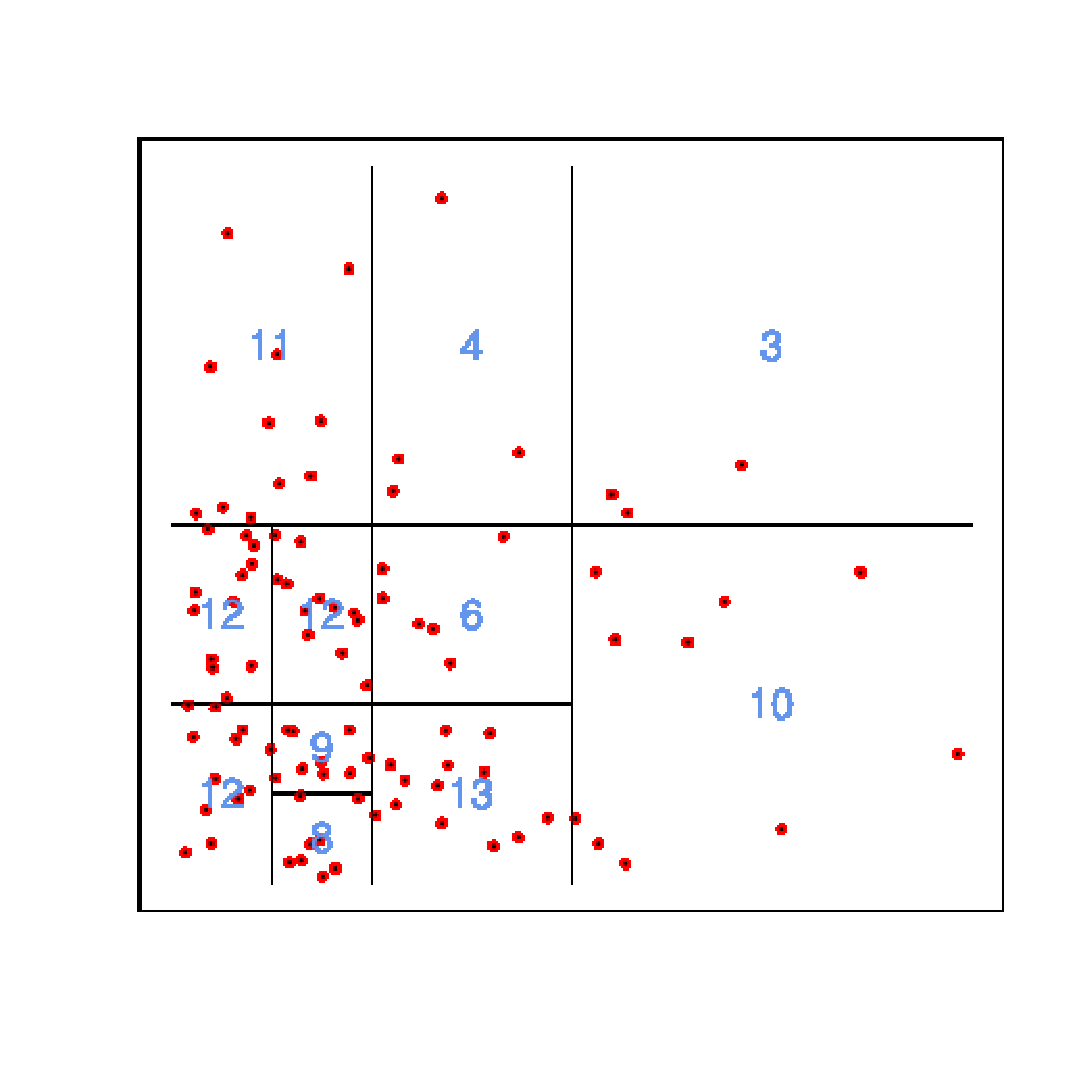
\includegraphics[width=0.3\textwidth]{norm_geom.eps}
	}
	\hspace{3pt}%
	\subfloat[][Cardinal Split]{%
		\label{norm:card}%
		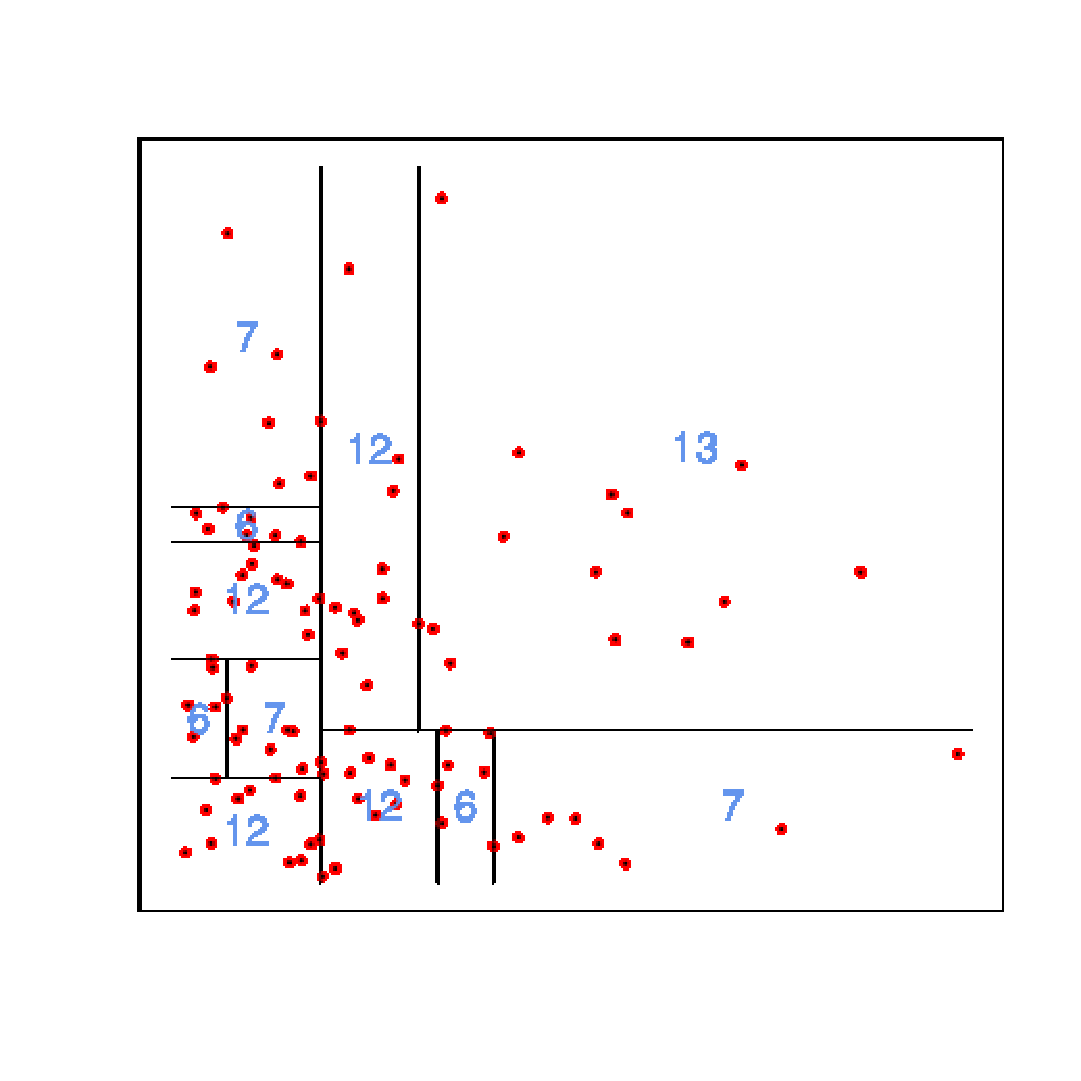
\includegraphics[width=0.3\textwidth]{norm_card.eps}
	}
	\hspace{3pt}%
	\subfloat[][Mean Split]{%
		\label{norm:mean}%
		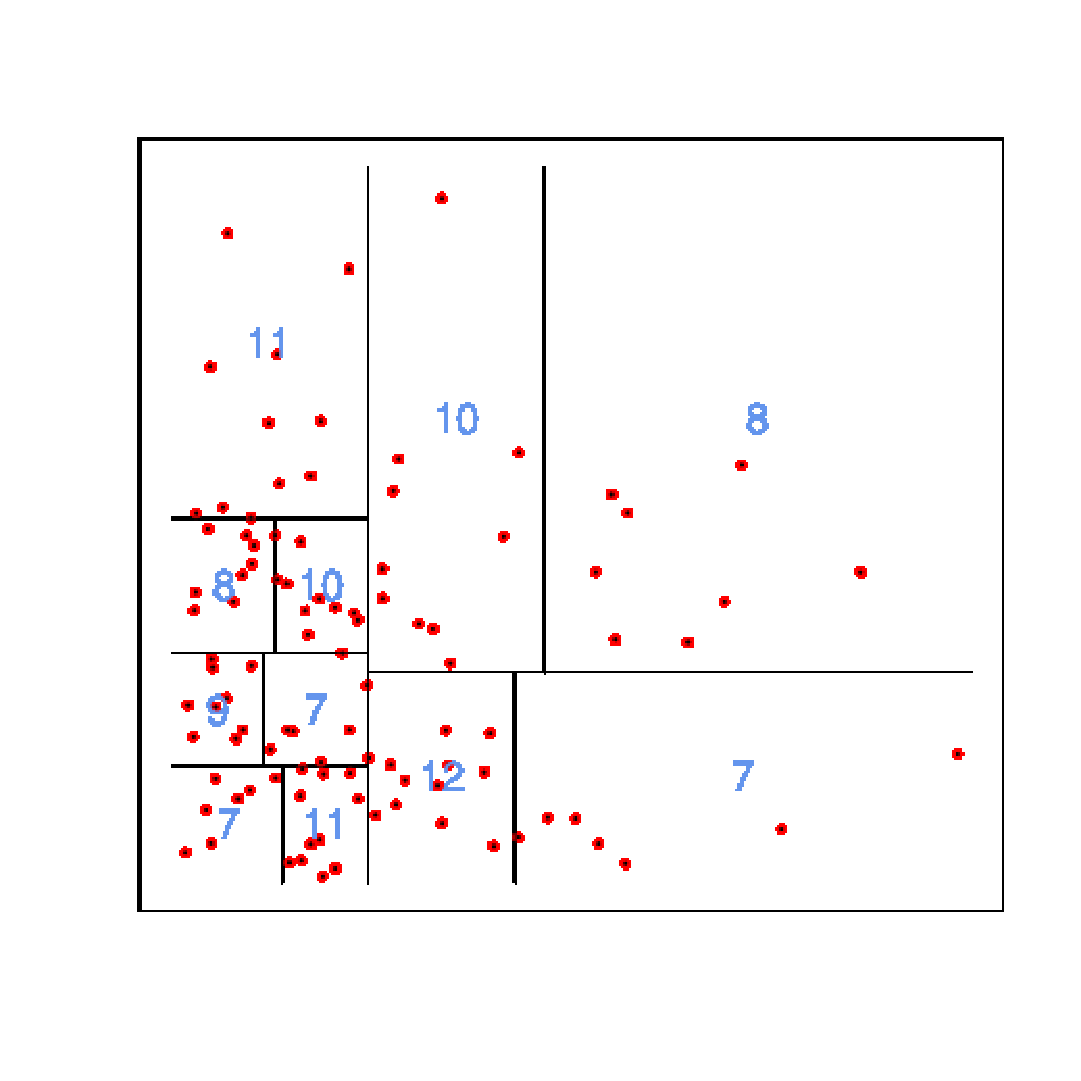
\includegraphics[width=0.3\textwidth]{norm_mean.eps}
	}
	\caption[]{Split domain of point normally distributed $\mathcal{N}\left(0,0.35\right)$}%
	\label{split:norm}
\end{figure}

\begin{figure}
	\centering
	\subfloat[][Geometrical Split]{
		\label{unif:geom}
		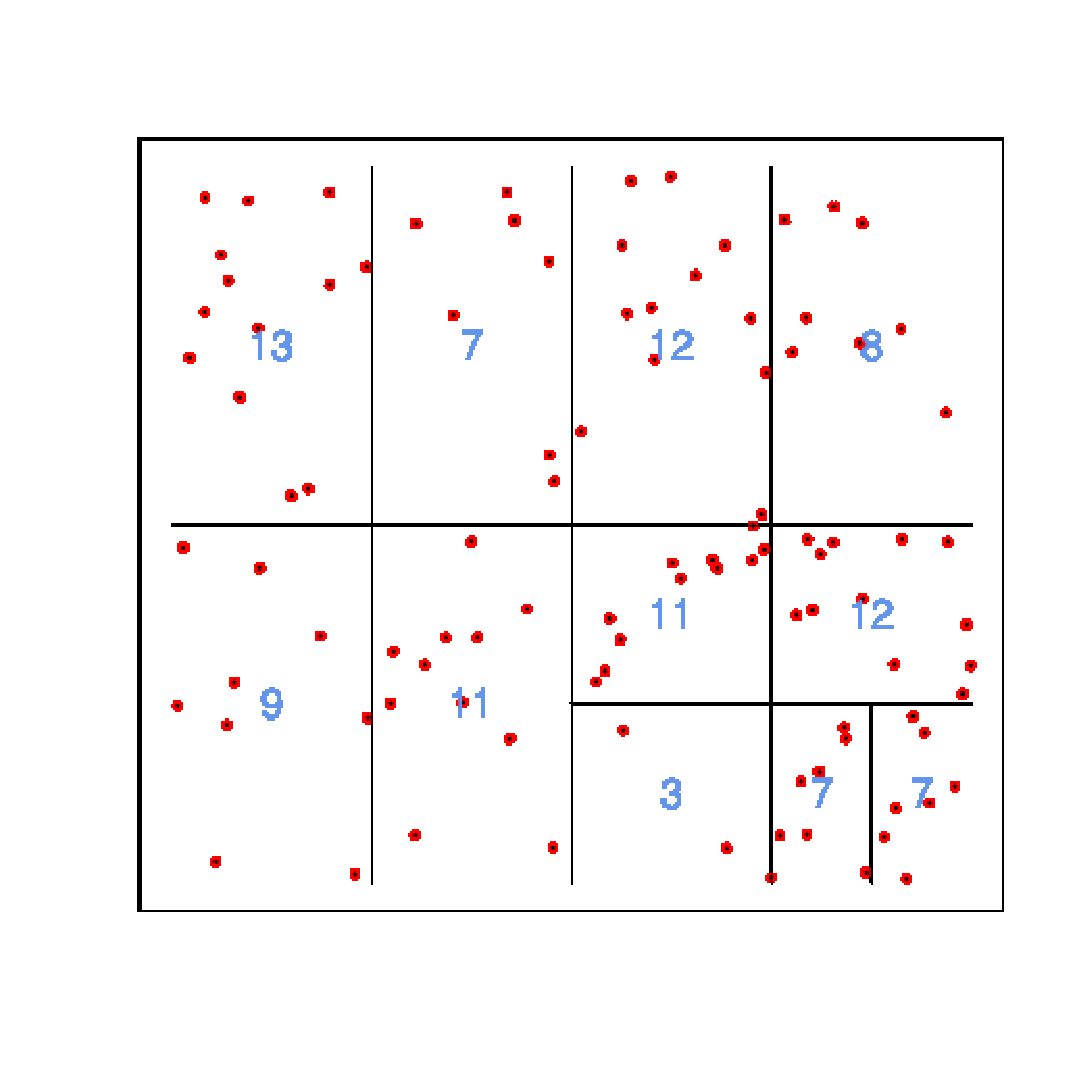
\includegraphics[width=0.3\textwidth]{unif_geom.eps}
	}
	\hspace{3pt}%
	\subfloat[][Cardinal Split]{%
		\label{unif:card}%
		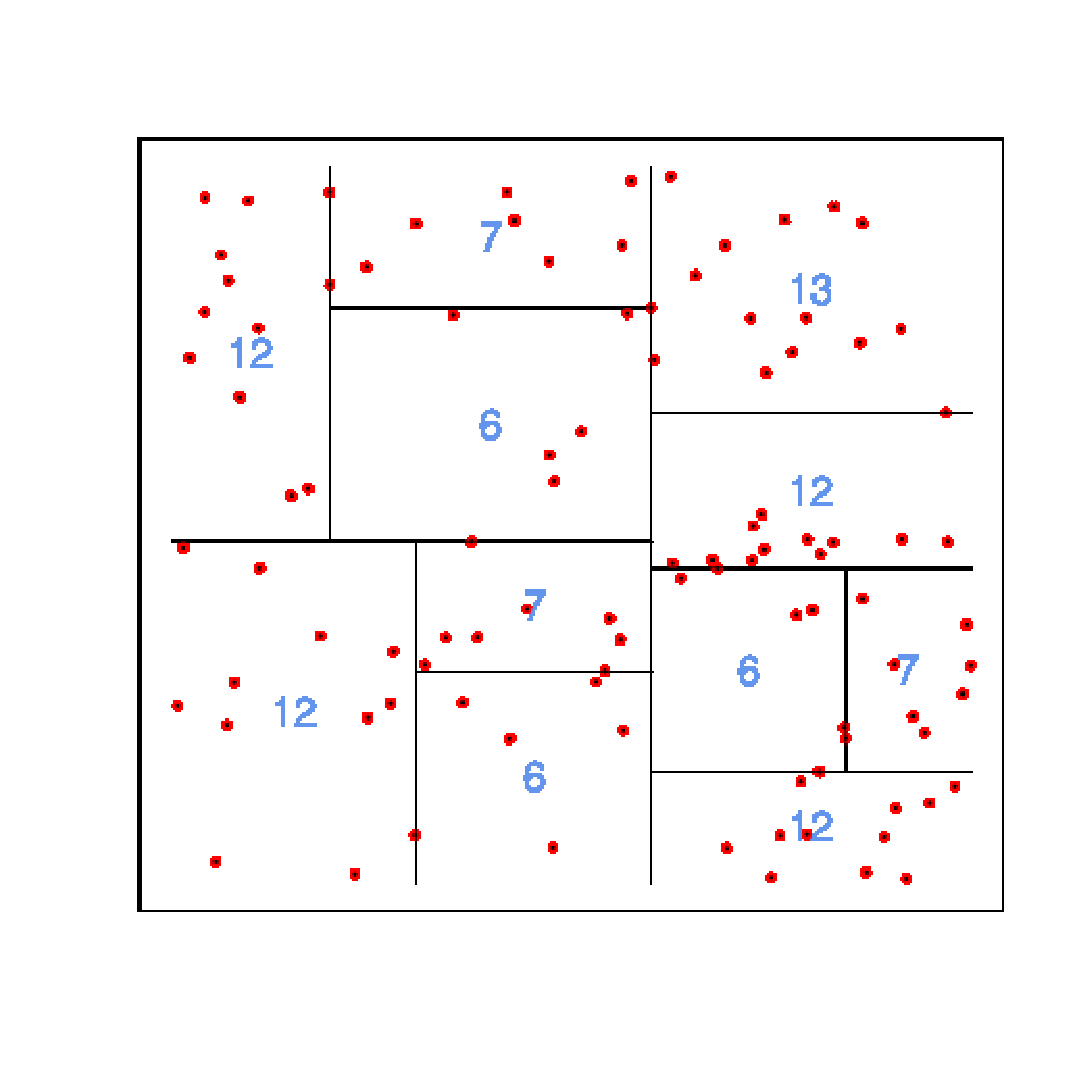
\includegraphics[width=0.3\textwidth]{unif_card.eps}
	}
	\hspace{3pt}%
	\subfloat[][Mean Split]{%
		\label{unif:mean}%
		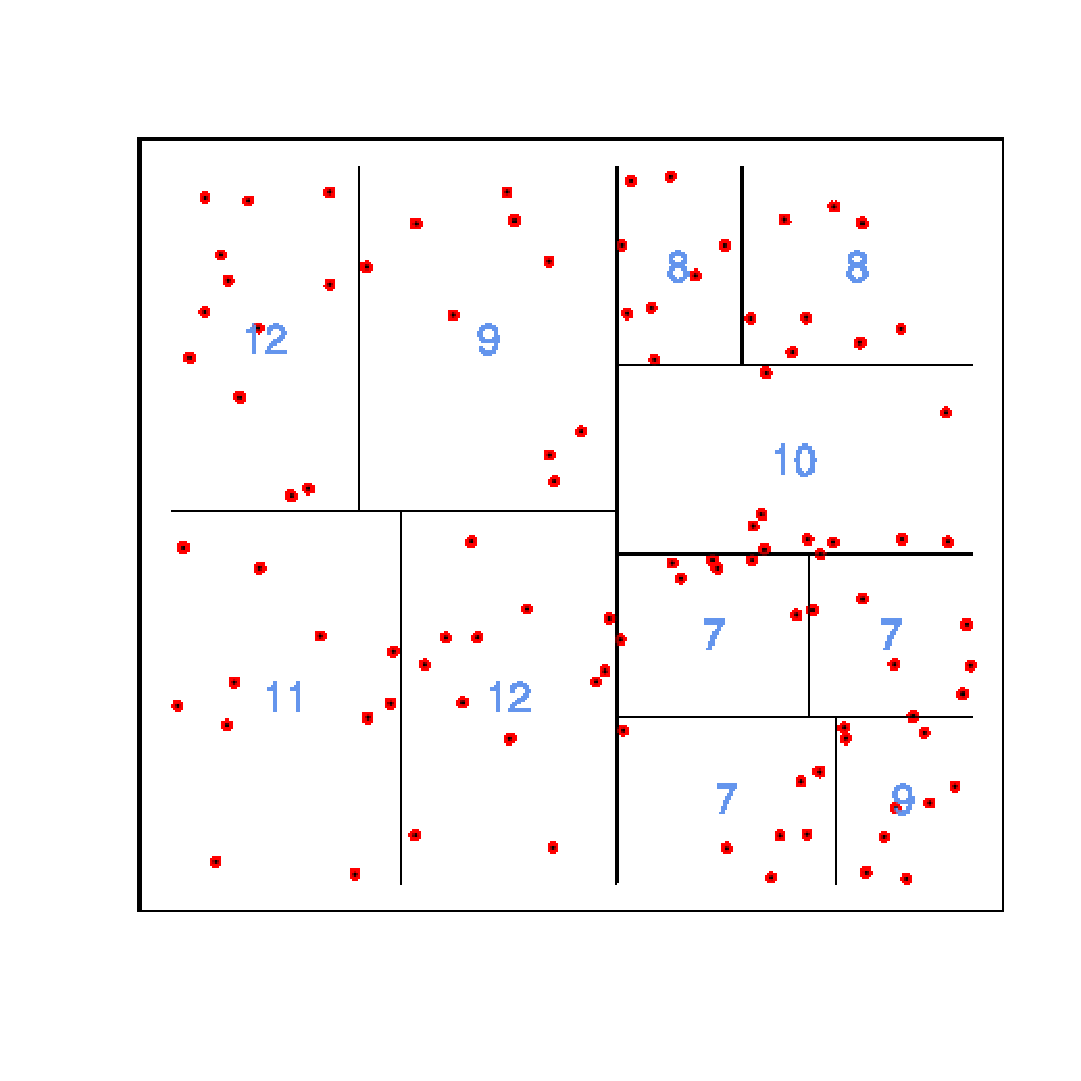
\includegraphics[width=0.3\textwidth]{unif_mean.eps}
	}
	\caption[]{Split domain of point uniformly distributed}%
	\label{split:unif}
\end{figure}

\begin{figure}
	\centering
	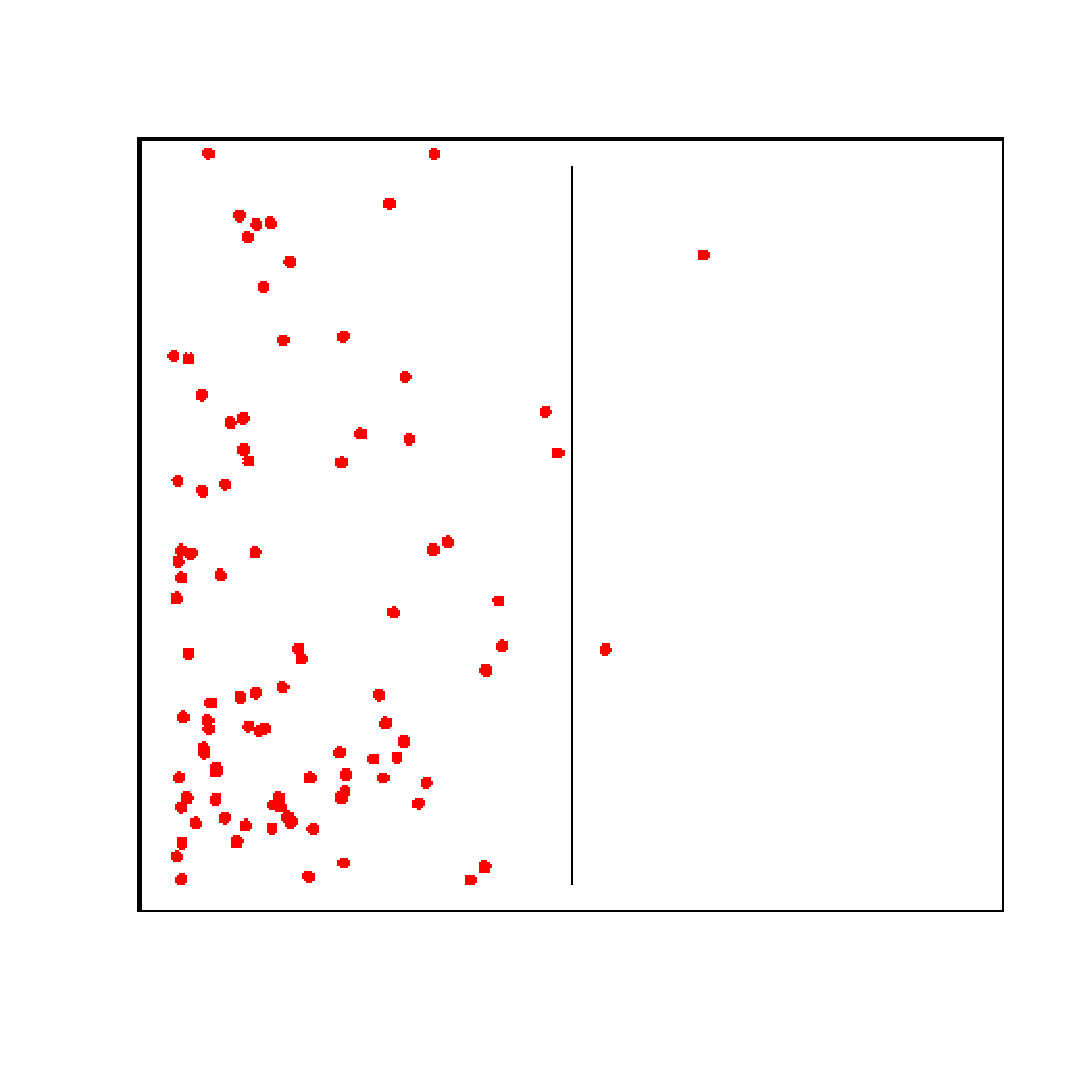
\includegraphics[width=0.3\textwidth]{badGeo.eps}
	\caption[]{If we assume $C = 3$ then this set can't be divided}%
	\label{fig:badGeom}
\end{figure}

\begin{enumerate}
\item {\bf Geometrical Split}: 
\begin{itemize}
\item \underline{Split criterion}: {\it Geometrical} $\rightarrow$ Dividing the region in tow parts with the same area.
\item \underline{Cut point}: The middle point of the x--axis (or y--axis, depending on the shape)
\item \underline{Result}: Two equal regions, but with different amount of clients (see Figure~\ref{norm:geom}). In the next step, the next sub-domain to divide will be, from those already divided, the most populated one (the sub-domain with more clients).
\item \underline{Problem}: Maybe we need to divide a sub-domain because it has a lot of client, but in the other hand it generate a sub-domain with a few clients, as you can see in the Figure~\ref{fig:badGeom}.
\item \underline{Benefit}: Very fast split. If we attack scenarios with point uniformly distributed, the behavior is pretty much desirable, as we can see in the Figure ~\ref{unif:geom}. 
\end{itemize}

\item {\bf Cardinal Split}
\begin{itemize}
\item \underline{Split criterion}: The number of clients, i.e., a sub-domain is divided in such a way that in the resulting sub-sub-domains there will be the same number of clients.
\item \underline{Cut point}: The current sub-domain is ordered and the x--axis (or y--axis, depending on the shape) of the element (location of the client) right in the center is selected to be the {\it cut point}
\item \underline{Result}: Two regions with the same ($\pm 1$) amount of clients (see Figure~\ref{norm:geom}). In the next step, the next sub-domain to divide will be, from those already divided, the most populated one (the sub-domain with more clients).
\item \underline{Problem}: The subdivision process is a bit more costly: we need to group the clients on both sides of a {\it perfect pivot}\footnote{Element of a set with the same number of elements lower and greater than him}.
\item \underline{Benefit}: It guarantees the same cardinality in both new sub-sub-domains.
\end{itemize}

\item {\bf Mean Split}
\begin{itemize}
\item \underline{Split criterion}: This is a mid-point strategy between the two previous. The goal is to find a {\it cut point} to group the elements of the current sub-domain, but in a easy way (fast), for that reason we do not compute the exact middle point to produce two sub-sub-domains with the same cardinality, as in the previous approach, instead of that we work with his expected value: the arithmetic mean.
\item \underline{Cut point}: We compute the mean of the $x$--axis (or $y$--axis) of the elements (locations) of the current sub-domain, and it will be the {\it cut point}
\item \underline{Result}: Two regions with not exact information about their sizes or their cardinality.
\item \underline{Problem}: {\it Idem.}
\item \underline{Benefit}: The {\it cut point} can be obtained by a $O(n)$ number of operations. As we can see in the preliminary results\footnote{The experiments are coded in R\cite{Paradis2005}.} (Figures~\ref{fig:goodMeanNorm} and \ref{fig:goodMeanUnif}), the behavior of this technique is near to the {\it cardinal split} technique, at least for normally and uniformly distributed sets of point.
\end{itemize}
\end{enumerate}

\begin{figure}
	\centering
	\subfloat[][Normally distributed]{
		\label{fig:goodCardNorm}
		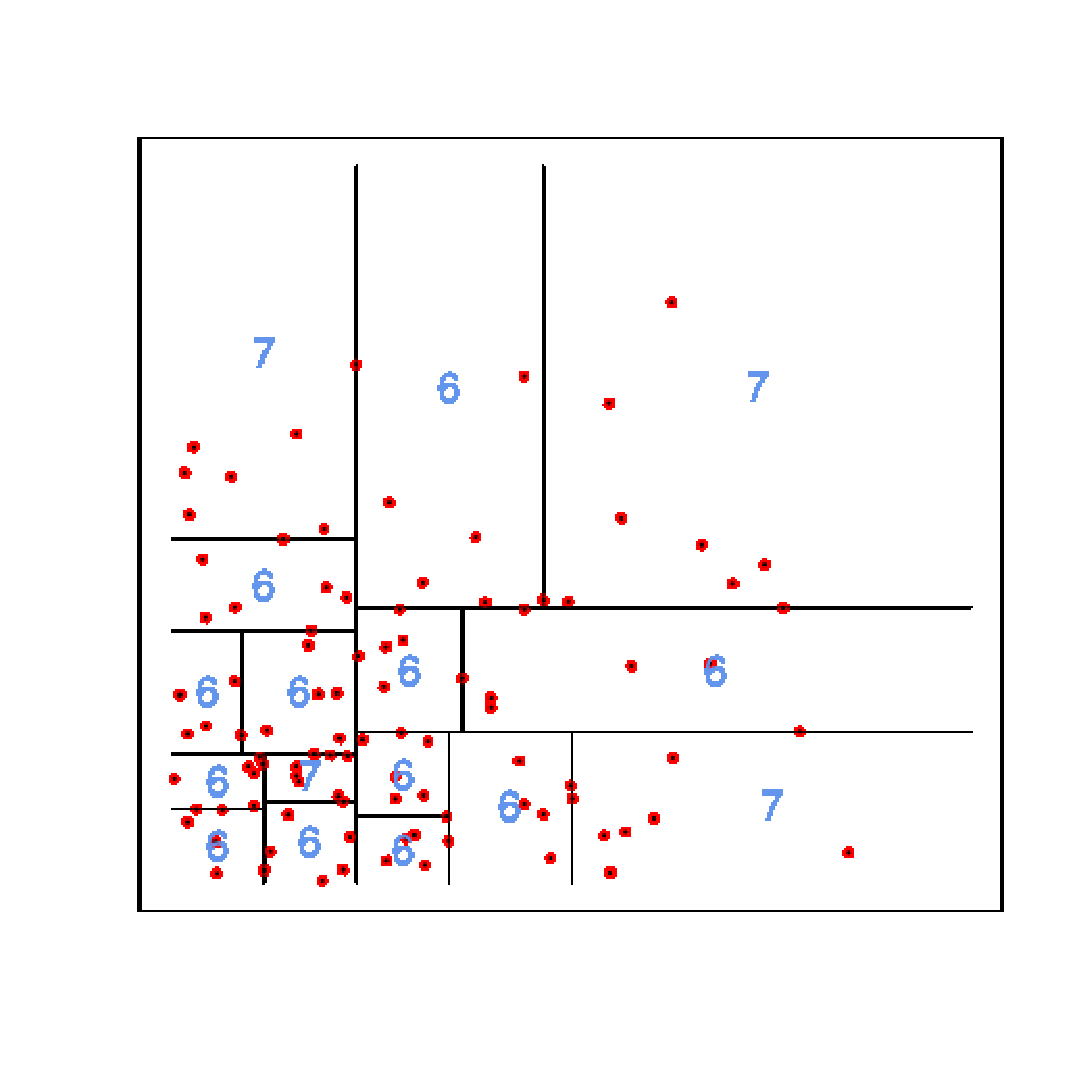
\includegraphics[width=0.3\textwidth]{goodCard.eps}
	}
	\hspace{3pt}%
	\subfloat[][Uniformly distributed]{%
		\label{fig:goodCardUnif}
		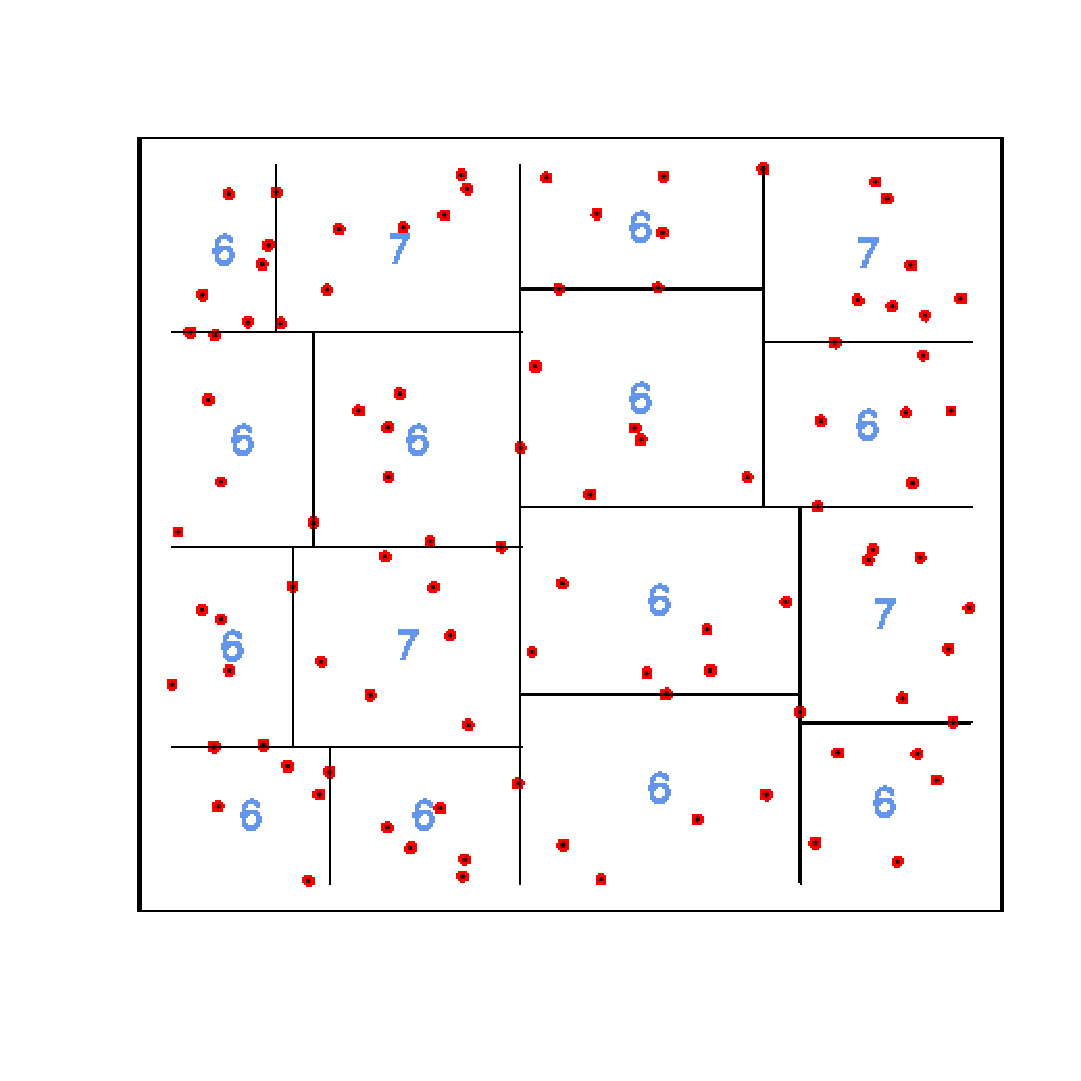
\includegraphics[width=0.3\textwidth]{goodCard2.eps}
	}\\
	\subfloat[][Normally distributed]{
		\label{fig:goodMeanNorm}
		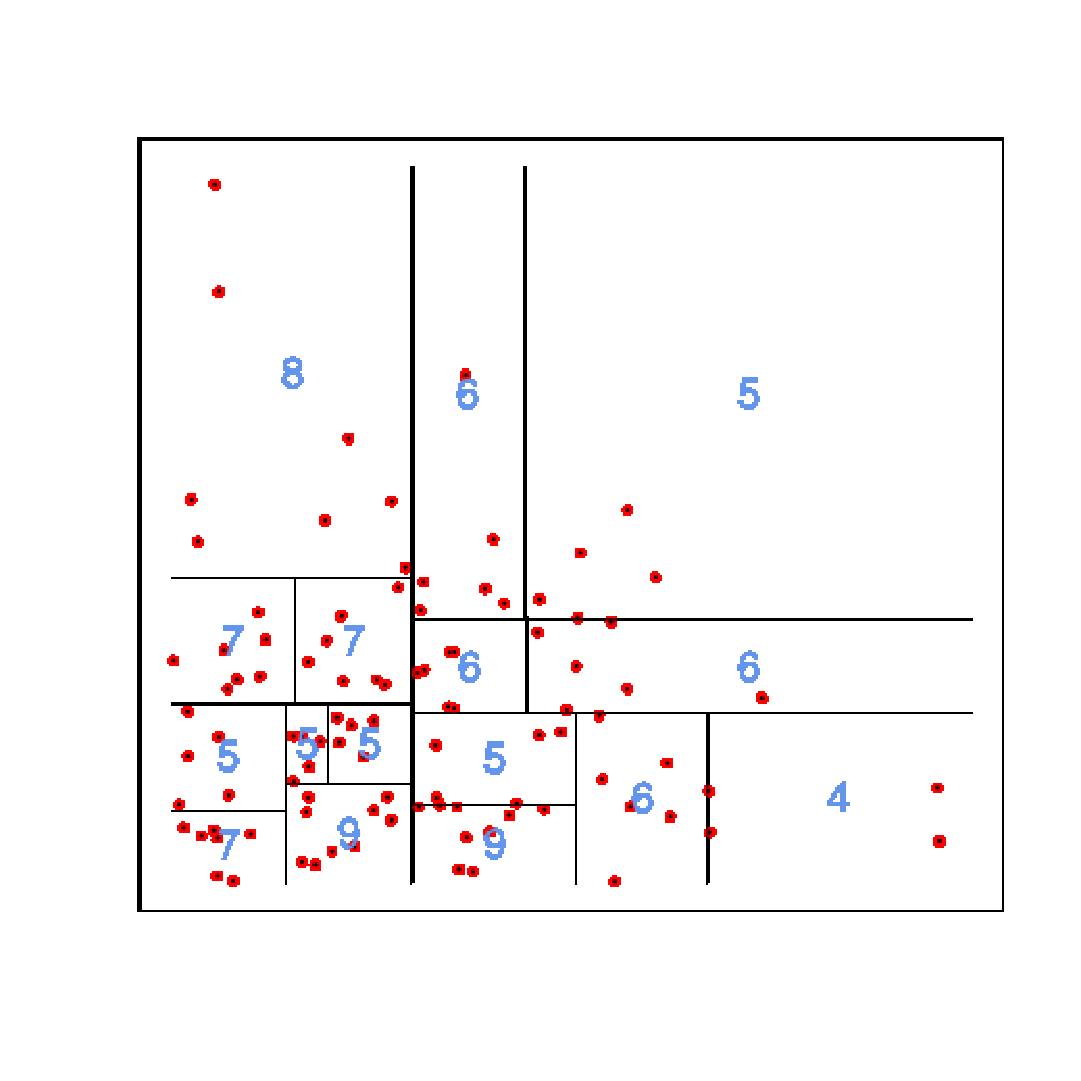
\includegraphics[width=0.3\textwidth]{goodMean.eps}
	}
	\hspace{3pt}%
	\subfloat[][Uniformly distributed]{%
		\label{fig:goodMeanUnif}
		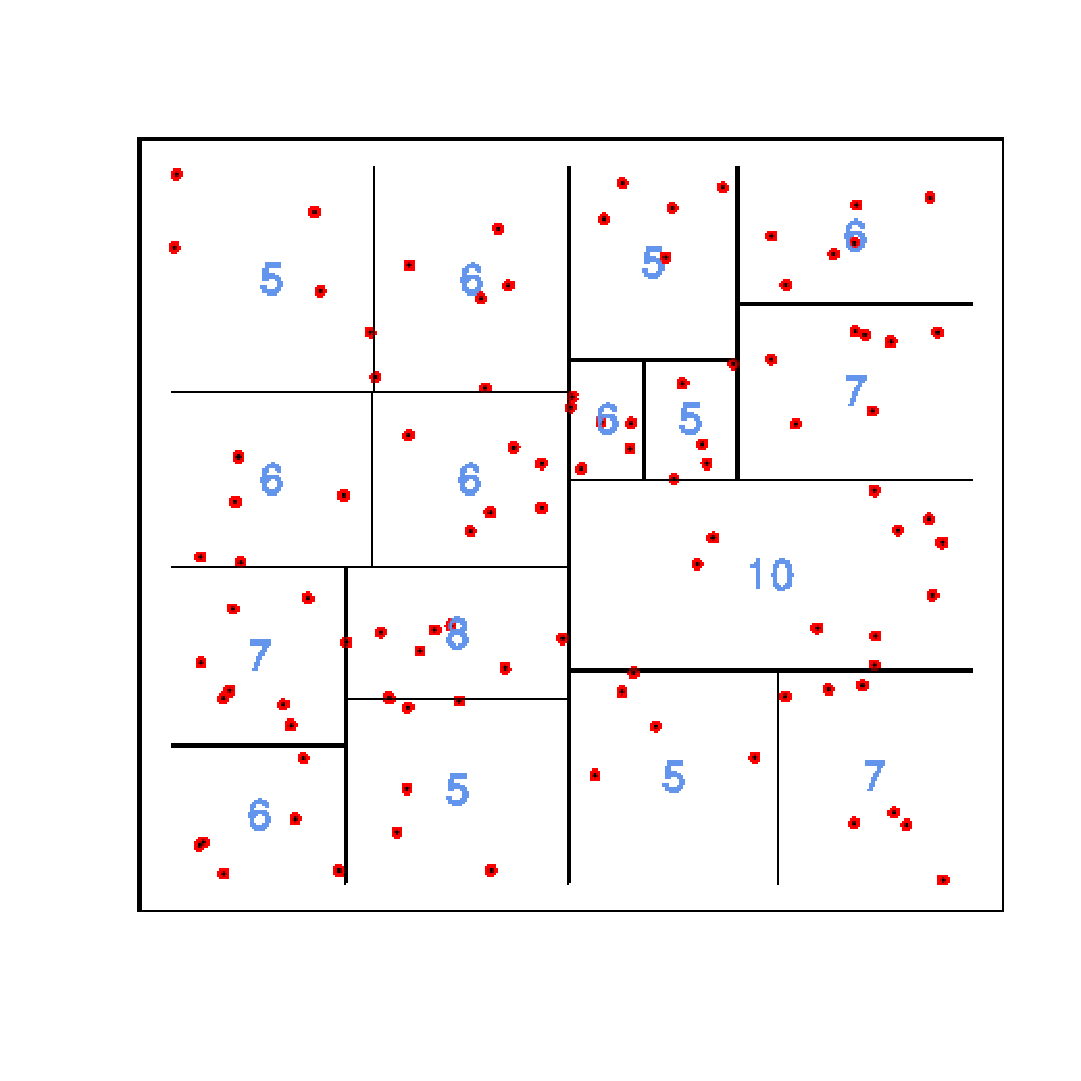
\includegraphics[width=0.3\textwidth]{goodMean2.eps}
	}
	\caption[]{Domain divided in $2^4 = 16$ sub-domains:
		\subref{fig:goodCardNorm} -
		\subref{fig:goodCardUnif} Cardinal;
		\subref{fig:goodMeanNorm} -	
		\subref{fig:goodMeanUnif} Mean.}%
	\label{fig:goodCard}
\end{figure}

%\textcolor{orange}{
%Is easy to see that this strategy guarantees that every built subset has at most two times the elements of some other. Let's take a look to the following example, but first we need to remember that: }
%
%\begin{itemize}
%\item \textcolor{orange}{The point is that every time we choose the most populated set to be divided}
%\item \textcolor{orange}{The current sub-domain is divided in two sub-sub-domains with the same cardinality.}
%\end{itemize} 
%
%\begin{example}
%\textcolor{orange}{
%This example will allow us to intuitively prove the above affirmation.}
%
%\textcolor{orange}{Suppose that there is a sub-domain $A$ in the list with more than two-times the number of element of some other and let's call it $B$. In other words:}
%
%$$\left| A\right| = 2\cdot k\cdot\left| B\right|$$
%$$\text{with } k \in \mathbb{Z}^+$$
%
%\textcolor{orange}{In that case, $B$ was built splitting some other with $\left(2\cdot (k-1)\cdot\left| B\right|\right)$ elements, and it was selected to be divided instead of $A$: \sc{Contradiction!!}}
%\end{example}
%
%\textcolor{orange}{This problem can be avoided forcing the algorithm to generate a quantity of sub-domains power of 2 (see Figure \ref{fig:goodCard}).}

\subsection{Conclusion}

In this section we present a theoretical and not validated work where we applied the {\it search space subdivision} approach to solve {\it k-medoids problem} in parallel. We have proposed some different strategies and we have showed graphically some characteristics of them. 

\section{Tunning methods for local search algorithms}
\label{sec:paramils}


%\textcolor{green}{
%My idea here is to present the work with ParamILS. I worked with the sets of training and test instances, and I think that the key is there, because I obtained a little change in the parameters configuration. The other point is that maybe Costas Array is not a good example to work, because the difference between the runs are too small. I hope that working with other problems, including more training instances, we can obtain better results.}

% short paragraph: about autotuning of parameters; work in progress.

In this section we present our results applying {\sc ParamILS} (version 2.3)\footnote{Open source program (project) in {\it Ruby}, available at \href{http://cs.ubc.ca/labs/beta/Projects/ParamILS}{\texttt{http://cs.ubc.ca/labs/beta/Projects/ParamILS}}}. {\sc ParamILS} (first introduced by Hutter, Hoos and St\:utzle in 2007), is a stochastic local search approach for automated algorithm configuration. The source is available on internet and includes some examples that you can run and see how the tool works. In addition, it brings a complete User Guide with a compact explanation about how to use it with a specific solver \cite{Hutter2008,Hutter2009}. In this study we used it to tune {\it Adaptive Search} solver\footnote{An implementation from Daniel D\'{i}az available at \href{https://sourceforge.net/projects/adaptivesearch/}{https://sourceforge.net/projects/adaptivesearch/}}. %It is an open source program (project) in {\it Ruby}, and the public source code include some examples and a detailed and complete \textit{User Guide} with a compact explanation about how to use it with a specific solver . 

The first step was building a {\it wrapper} in C++ language, in order to tune more than one problem with the same code. The goal of doing this is using the tool to tune the solver, i.e., finding the best parameter configuration for a specific problem, but also the best parameter configuration to solve any kind of benchmark (a general parameter configuration).

\nocite{Rickard}

Following we present in Table~\ref{table:param} the parameter list that we worked with:

\begin{table}[ht] 
\caption{Adaptive Search parameters}
\centering 
\begin{tabular}{c c l}
\hline\hline
Parameter & Type & Description \\ [0.5ex]
\hline
-P & PERCENT & probability to select a local min (instead of staying on a plateau) \\
-f & NUMBER & freeze variables of local min for NUMBER swaps \\ 
-F & NUMBER & freeze variables swapped for NUMBER swaps \\ 
-l & LIMIT & reset some variables when LIMIT variable are frozen \\ 
-p & PERCENT & reset PERCENT of variables \\ [1ex]
\hline
\end{tabular} 
\label{table:param}
\end{table} 

In this section, we explain in details the implementation and the experimentation process.

\subsection{Using ParamILS}

To use the tool {\sc ParamILS}, we have installed Ruby! 1.8.7 in our computer. We used a laptop \mylaptopName (\mylaptopProc, \mylaptopMemo) with {\sc Ubuntu~14.4}. To run the tool, we needed to use the following command line:

\begin{BGVerbatim}
>> ruby param_ils_2_3_run.rb -numRun 0 -scenariofile /.../<scenario_file> -validN 100
\end{BGVerbatim}

Where \texttt{$<$scenario\_file$>$} is the name of the file where we have to put all the information that {\sc ParamILS} needs to tune the solver (the \textit{tuning scenario file}). We explain its content in the next section.

\subsection{Tuning scenario files}

The {\it tuning scenario file} is a text file with all needed information to tune the solver using {\sc ParamILS}. It includes where to find the solver binary file, the parameters domains, etc. In our case, the {\it tuning scenario file} looks like the following:

\begin{shadedbox}
	\texttt{algo = ./QtWrapper\_wrapper\\
		execdir = /.../src \\
		deterministic = 0 \\
		run\_obj = runtime \\
		overall\_obj = mean \\
		cutoff\_time = 50.0 \\
		cutoff\_length = max \\
		tunerTimeout = 3600 \\
		paramfile = instances/all\_intervals-params.txt \\
		outdir = instances/all\_intervals-paramils-out \\
		instance\_file = instances/.../all\_intervals-lower-instances.txt \\
		test\_instance\_file = instances/.../all\_intervals-upper-instances.txt \\
	}
\end{shadedbox}

We explain in details each line in this file:

\begin{itemize}
	\item \textbf{\texttt{algo}} $\rightarrow$ An algorithm executable or a call to a wrapper script around an algorithm that aims the input/output format of \textit{ParamILS} (the wrapper).
	\item \textbf{\texttt{execdir}} $\rightarrow$ Directory to execute \textbf{\texttt{algo}} from: "cd $<$\texttt{execdir}$>$; $<$\texttt{algo}$>$" 
	\item \textbf{\texttt{run\_obj}} $\rightarrow$ A scalar quantifying how "good" a single algorithm execution is, such as its required runtime.
	\item \textbf{\texttt{overall\_obj}} $\rightarrow$ While \textbf{\texttt{run\_obj}} defines the objective function for a single algorithm run, \textbf{\texttt{overall\_obj}} defines how those single objectives are combined to reach a single scalar value to compare two parameter configurations. Implemented examples include {\bf mean}, {\bf median}, {\bf q90} (the 90\% quantile), {\bf adj\_mean} (a version of the mean accounting for unsuccessful runs: total runtime divided by number of successful runs), {\bf mean1000} (another version of the mean accounting for unsuccessful runs: (total runtime of successful runs + 1000 x runtime of unsuccessful runs) divided by number of runs -- this effectively maximizes the number of successful runs, breaking ties by the runtime of successful runs; it is the criterion used in most of Frank experiments), and {\bf geomean} (geometric mean, primarily used in combination with \textbf{\texttt{run\_obj}} = \texttt{speedup}. The empirical statistic of the cost distribution (across multiple instances and seeds) to be minimized, such as the mean (of the single run objectives). \footnote{We use {\bf mean} but maybe we can experiment with other values}
	\item \textbf{\texttt{cutoff\_time}} $\rightarrow$ The time after which a single algorithm execution will be terminated unsuccessfully. This is an important parameter: if chosen too high, lots of time will be wasted with unsuccessful runs. If chosen too low the optimization is biased to perform well on easy instances only.
	\item \textbf{\texttt{tunerTimeout}} $\rightarrow$ The timeout of the tuner. Validation of the final best found parameter configuration starts after the timeout.
	\item \textbf{\texttt{paramfile}} $\rightarrow$ Specifies the file with the parameters of the algorithms. 
	\item \textbf{\texttt{outdir}} $\rightarrow$ Specifies the directory \textit{ParamILS} should write its results to.
	\item \textbf{\texttt{instance\_file}} $\rightarrow$ Specifies the file with a list of training instances. 
	\item \textbf{\texttt{test\_instance\_file}} $\rightarrow$ Specifies the file with a list of test instances.
\end{itemize}

Another important file that we have to compose properly is the {\it algorithm parameter file}, just following the instruction from \cite{Hutter2008} --\textit{[...] each line lists one parameter, in curly parentheses the possible values considered, and in square parentheses the default value [...]}. Our {\it algorithm parameter file} looks like follows:\\

\begin{shadedbox}
	\texttt{P \{20, 25, 30, 35, 40, 45, 50, 55, 60\} [50]\\
		f \{0, 1, 2, 3\} [1]\\
		F \{0, 1, 2, 3\} [0]\\
		l \{0, 1, 2, 3\} [1]\\
		p \{1, 2, 3, 5, 10, 20\} [5]
	}
\end{shadedbox}

In the current {\it Adaptive Search} implementation, the solver binary file and the problem instance are the same thing. It means that we only have to use the following command to solve the {\it All--intervals} problem of size $K$, for example: 

\begin{BGVerbatim}
>> ./all-intervals K
\end{BGVerbatim}

So, to use {\sc ParamILS} we modified a little the code: now our solver takes the size parameter from a text file. That way, the instance file is a text file only containing a number.

The solver we want to tune using {\sc ParamILS} ({\it Adaptive Search} in this case), must aims specific input/output rules. For that reason instead of modifying the current code of {\it Adaptive Search} implementation, we preferred to build a wrapper.

\subsection{Building the wrapper}

The algorithm executable must follow the input/output criteria presented below: 

\textbf{\large Launch command:} 

\begin{BGVerbatim}
>> <algo_exectuable> <instance_name> <instance-specific_information> ...
<cutoff_time> <cutoff_length> <seed> <params>
\end{BGVerbatim}

\begin{itemize}
	\item \texttt{$<$algo\_exectuable$>$} Solver 
	\item \texttt{$<$instance\_name$>$} In our case, a text file containing only the problem size
	\item \texttt{$<$instance-specific\_information$>$} We don't use it 
	\item \texttt{$<$cutoff\_time$>$} Cut off time for each run of the solver (see above)
	\item \texttt{$<$cutoff\_length$>$} We don't use it
	\item \texttt{$<$seed$>$} Random seed
	\item \texttt{$<$params$>$} Parameters and its values
\end{itemize}

\underline{Exmaple:}

\begin{BGVerbatim}
>> ./QtWrapper_320.txt "" 50.0 214483647 524453158 -p 5 -l 1 -f 1 -P 50 -F 0
\end{BGVerbatim}

\textbf{\large Output:} 

\begin{BGVerbatim}
>> <solved>, <runtime>, <runlength>, <best_sol>, <seed>
\end{BGVerbatim}

\begin{itemize}
	\item {\bf $<$solved$>$} \texttt{SAT} if the algorithm terminates successfully. \texttt{TIMESOUT} if the algorithm times out.
	\item {\bf $<$runtime$>$} Runtime
	\item {\bf $<$runlength$>$} -1 (as Frank Hutter recommended)
	\item {\bf $<$best\_sol$>$} -1 (as Frank Hutter recommended)
	\item {\bf $<$cutoff\_length$>$} We don't use it
	\item {\bf $<$seed$>$} Used random seed
\end{itemize}

\underline{Exmaple:}

\begin{BGVerbatim}
>> SAT, 2.03435, -1, -1, 524453158
\end{BGVerbatim}

To build the wrapper we have followed a simple algorithm: launch two concurrent process. In the parent process we translate the input of the wrapper to the input of {\it Adaptive Search} solver. The solver is executed, and the runtime is measured. After that we post the output properly. In the child process a {\it sleep} command is executed for \texttt{$<$runtime$>$} seconds and after that, if the parent process has not finished yet, it is killed, posting a time-out message. See Algorithm~\ref{wrapper} for more details.

%\incmargin{1.4em}
\linesnumbered
\begin{algorithm}[H]
	\caption{Costas Wrapper}
	\label{wrapper}
	\dontprintsemicolon
	\SetLine
	\SetKwData{paramConfig}{$\theta$}
	\SetKwData{seed}{s}
	\SetKwData{Inst}{$Pth_{\pi}$}
	\SetKwData{cotime}{$k$}
	\SetKwData{pilsOut}{$PiLS_{out}$}
	\SetKwData{tstart}{$t_0$}
	\SetKwData{tend}{$t_e$}
	\SetKwData{timet}{$t$}
	\SetKwData{strCal}{strCall}
	\SetKwFunction{fork}{fork}
	\SetKwFunction{TIC}{clock\_TIC}
	\SetKwFunction{TOC}{clock\_TOC}
	\SetKwFunction{buildStr}{build\_str}
	\SetKwFunction{call}{systemCall}
	\SetKwFunction{kill}{killProcess}
	\SetKwFunction{output}{paramilsOutput}
	\SetKwFunction{sleep}{sleep}
	\SetKwInOut{Input}{input}
	\SetKwInOut{Output}{output}
	
	\Input{\Inst : problem instance path, \cotime : cut off time, \seed : random seed, \paramConfig : parameters configuration}
	\Output{\pilsOut : Output in a {\sc ParamILS} way}
	\BlankLine
	
	\fork{} \tcc{Divide the execution in two processes}
	\eIf{$<$in child process$>$}{
		\tstart $\leftarrow$ \TIC{}\;
		\strCal $\leftarrow$ \buildStr{\texttt{" ./AS\_Wrapper \%1 -s \%2 \%3"}, \Inst, \seed, \paramConfig}\;
		\call{\strCal}\;
		\tend $\leftarrow$ \TOC{}\;
		\kill{$<$parent process$>$} \label{paso7}\;
		\timet $\leftarrow$ \tend - \tstart\;
		{\bf return} \output{SAT, \timet, \seed}\;
	}{
	\sleep{\cotime}\;
	\kill{$<$child process$>$}\;
	{\bf return} \output{TIMESOUT, \cotime, \seed}\;
}
\end{algorithm}

\subsection{Using the wrapper}

In this section we explain how to use our wrapper to be able to tune easily instances of {\it All-Interval Series} and \carr{} problems. The {\it All-Interval Series Problem}\footnote{CSPlib:007 (\href{http://www.csplib.org/Problems/prob007/}{\texttt{http://www.csplib.org/Problems/prob007/}})} is the problem of finding a vector $s=\left(s_1,\dots,s_n\right)$, given $n \in \mathbb{N}$, such that $s$ is a permutation of the vector $(0, 1, \dots, n-1)$ and the interval vector $v = \left(\left|S_2-s_1\right|, \left|S_3-s_2\right|, \dots, \left|S_n-S_{n-1}\right|\right)$ (called an all-interval series of size $n$) is a permutation of the vector $(1, 2, \dots, n-1)$. The \carrp{} consists in finding a Costas array, which is an $n\times n$ grid containing $n$ marks such that there is exactly one mark per row and per column and the $n(n-1)/2$ vectors joining each couple of marks are all different (see below for more details about this problems).

\subsubsection{Factory call}

The first step is to implement the class {\sc ICallFactory}. Here, the string-binary-name for the command call is statically obtained. We present, as example, the class {\sc All\_IntervalCallFactory}:

\begin{Verbatim}[fontsize=\normalsize]
\textcolor{verde}{\bf// all_interval_call_factory.h}
\textcolor{blue}{\bf class} All_IntervalCallFactory: \textcolor{blue}{\bf public} ICallFactory
\{
   \textcolor{blue}{\bf public}:
      std::string BuildCall();
      std::string BuildDefaultCall();
\};
\end{Verbatim}

\begin{Verbatim}[fontsize=\normalsize]
\textcolor{verde}{\bf// all_interval_call_factory.cpp}
\textcolor{dred}{\bf #define} ALGO_EXECUTABLE "./all-interval"
\textcolor{dred}{\bf #define} DEFAULT_CALL "./all-interval _100.txt"

std::string All_IntervalCallFactory::BuildCall()
\{
   \textcolor{blue}{\bf return} ALGO_EXECUTABLE;
\}
std::string All_IntervalCallFactory::BuildDefaultCall()
\{
   \textcolor{blue}{\bf return} DEFAULT_CALL;
\}
\end{Verbatim}

All we have to do is to define our new macro {\bf ALGO\_EXECUTABLE} ({\bf DEFAULT\_CALL} is not being used)

\subsubsection{Main method}

Let's suppose now that we want to run an algorithm called {\it mySolver} that receives a file as parameter, called {\it my\_instance\_size.txt} (this is mandatory). We have to create (as we've explained before) the class {\sc My\_SolverCallFactory} and defining the macro as follows:

\begin{Verbatim}[fontsize=\normalsize]
\textcolor{dred}{\bf #define} ALGO_EXECUTABLE "./mySolver"
\end{Verbatim}

Now, the main method would be exactly like this:

\begin{Verbatim}[fontsize=\normalsize]
\textcolor{blue}{\bf int} main(\textcolor{blue}{\bf int} argc, \textcolor{blue}{\bf char}* argv[])
\{
   shared_ptr<ICallFactory> problem = 
      make_shared<My_SolverCallFactory>();
   shared_ptr<TuningData> td = 
      (make_shared<TuningData>(argc, argv, problem));

   shared_ptr<ADWrapper> w (make_shared<ADWrapper>());
   string output = w->tune(td);

   cout << output << endl;
   \textcolor{blue}{\bf return} 0;
\}
\end{Verbatim}

\subsection{Results}

In this section we present the results of applying {\sc ParamILS} to the resolution of {\it All-Interval Series} and \carr{} problems through {\it Adaptive Search}. In both cases, we need to chose a set of {\it training instances}, to train the tuner, and a set of {\it test instances}, used to obtain the parameter setting. 

\subsubsection{ Tuning {\it Adaptive Search} for  {\it All-Intervals Series Problem}}

\underline{Study cases:}
\begin{enumerate}
	\item The {\it training instances set} is composed by instances of {\it All--Intervals} problems of order $N$ with $$N \in \left\{100, 110, 120, 130, 140, 150, 160, 170, 180\right\}$$
	\item The {\it test instances set} is composed by instances of {\it All--Intervals} problems of order $N$ with $$N \in \left\{190, 200, 210, 220, 230, 240, 250, 260, 265\right\}$$
	\item The time-out for each run is 50.0 seconds
	\item The test quality is based on 100 runs
\end{enumerate}

In a {\bf First Experiment} we use the following {\it parameters domains}:
\begin{itemize}[itemsep=0.2mm]
	\item {\bf P}\texttt{ \{41, 46, 51, 56, 60, 66, 71, 76, 80\}}
	\item {\bf F, f, l}\texttt{ \{0, 1, 2, 3\}}
	\item {\bf p}\texttt{ \{5, 10, 15, 20, 25, 30, 35\}}
\end{itemize}

Table~\ref{table:allint5yh} shows results using a time-out of 5.5 hours (20,000 seconds), and Table~\ref{table:allint1h} shows results using a time-out of 1 hour. In the second case we where able to perform more runs, due to the available time, but in both cases the training qualities are not so different. However, we can se the difference int the test qualities, and conclude that results using 5 hours of time-out are more reliables. 

\begin{table}[h] 	
\centering 
\renewcommand{\arraystretch}{1.2}
\resizebox{\columnwidth}{!}{%
\tablePILSresults{
	0 & 66 & 1 & 1 & 25 & 0 & 80 & 2 & 1 & 35 & 0.79666 & 1780 & 8.274 \\
	2 & 56 & 2 & 2 & 20 & 1 & 80 & 1 & 1 & 10 & 0.795 & 1637 & 5.508 \\
	0 & 41 & 0 & 0 & 5 & 1 & 80 & 3 & 0 & 15 & 0.789 & 1547 & 5.8478 \\
	3 & 80 & 3 & 3 & 35 & 1 & 80 & 2 & 0 & 10 & 0.880686 & 1258 & 6.15398\\
}
}
\caption{{\it All-Intervals Series}: \texttt{tunerTimeout} = 20,000 seconds}\label{table:allint5yh}
\end{table}

\begin{table}[h] 	
\centering 
\renewcommand{\arraystretch}{1.2}
\resizebox{\columnwidth}{!}{%
\tablePILSresults{
	0 & 66 & 1 & 1 & 25 & 0 & 80 & 0 & 1 & 25 & 0.815 & 384 & 5.8191 \\
	0 & 66 & 1 & 1 & 25 & 1 & 80 & 1 & 1 & 35 & 0.737 & 452 & 6.267 \\
	0 & 66 & 1 & 1 & 25 & 1 & 56 & 0 & 1 & 35 & 1.03 & 371 & 9.056 \\
	0 & 66 & 1 & 1 & 25 & 0 & 76 & 0 & 1 & 20 & 0.814 & 385 & 4.915 \\
	0 & 66 & 1 & 1 & 25 & 0 & 80 & 3 & 1 & 20 & 0.76 & 469 & 5.417 \\ 
	\hline
	2 & 56 & 2 & 2 & 20 & 0 & 41 & 0 & 1 & 10 & 0.919 & 239 & 18.364 \\
	2 & 56 & 2 & 2 & 20 & 0 & 56 & 1 & 1 & 20 & 0.819 & 407 & 5.409 \\
	2 & 56 & 2 & 2 & 20 & 1 & 80 & 1 & 1 & 35 & 0.772 & 457 & 5.43 \\
	2 & 56 & 2 & 2 & 20 & 1 & 80 & 0 & 1 & 10 & 0.858 & 504 & 5.566 \\
	2 & 56 & 2 & 2 & 20 & 0 & 80 & 1 & 1 & 10 & 0.7845 & 562 & 18.944 \\
	\hline
	0 & 41 & 0 & 0 & 5 & 0 & 41 & 1 & 0 & 10 & 0.9749 & 367 & 5.97813 \\
	0 & 41 & 0 & 0 & 5 & 0 & 41 & 1 & 0 & 10 & 0.885 & 450 & 5.706 \\
	0 & 41 & 0 & 0 & 5 & 0 & 41 & 1 & 0 & 10 & 0.906 & 335 & 18.707 \\
	0 & 41 & 0 & 0 & 5 & 0 & 41 & 1 & 0 & 10 & 0.995 & 335 & 19.558 \\
	0 & 41 & 0 & 0 & 5 & 0 & 41 & 0 & 0 & 5 & 0.855 & 404 & 5.686 \\
	\hline
	3 & 80 & 3 & 3 & 35 & 0 & 66 & 3 & 1 & 25 & 0.9118 & 230 & 26.585 \\
	3 & 80 & 3 & 3 & 35 & 0 & 80 & 1 & 1 & 10 & 0.732 & 310 & 7.875 \\
	3 & 80 & 3 & 3 & 35 & 0 & 80 & 0 & 1 & 20 & 0.816 & 303 & 7.2896 \\
	3 & 80 & 3 & 3 & 35 & 1 & 80 & 3 & 1 & 35 & 0.821 & 327 & 6.812 \\
	3 & 80 & 3 & 3 & 35 & 0 & 80 & 0 & 1 & 30 & 0.9203 & 443 & 5.401 \\
} 
}
\caption{{\it All-Intervals Series}: \texttt{tunerTimeout} = 3,600 seconds}\label{table:allint1h}
\end{table}

In a {\bf Second Experiment} we decide to enlarge a bit more the parameters domains and use a time-out of 5 hours. The {\bf Parameters domains} are the following:
\begin{itemize}[itemsep=0.2mm]
	\item {\bf P}\texttt{ \{10, 20, 30, 40, 50, 60, 70, 80, 90\}}
	\item {\bf F, f, l}\texttt{ \{0, 1, 2, 3, 4, 5, 6, 7, 8\}}
	\item {\bf p}\texttt{ \{10, 20, 30, 40, 50, 60, 70\}}
\end{itemize}

\begin{table}[h] 	
\centering 
\renewcommand{\arraystretch}{1.2}
\resizebox{\columnwidth}{!}{%
\tablePILSresults{
	0 & 10 & 0 & 0 & 10 & 0 & 40 & 7 & 0 & 50 & 0.883188 & 936 & 6.3191 \\
	0 & 10 & 0 & 0 & 10 & 0 & 80 & 2 & 1 & 40 & 0.774659 & 1584 & 5.45674 \\ 
	0 & 10 & 0 & 0 & 10 & 0 & 40 & 2 & 0 & 10 & 0.96885 & 1104 & 6.82643 \\ 
	\hline
	4 & 60 & 4 & 4 & 40 & 0 & 60 & 8 & 1 & 40 & 0.90358 & 1566 & 5.48127 \\
	4 & 50 & 4 & 4 & 40 & 0 & 80 & 5 & 1 & 20 & 0.78536 & 1662 & 11.5649 \\
	3 & 50 & 4 & 2 & 30 & 0 & 90 & 6 & 1 & 70 & 0.79440 & 1395 & 5.08108 \\
	\hline
	0 & 90 & 0 & 0 & 10 & 1 & 90 & 6 & 1 & 10 & 0.859569 & 1379 & 5.4286 \\ 
	0 & 90 & 0 & 0 & 10 & 1 & 90 & 6 & 1 & 30 & 0.80738 & 1117 & 5.47126 \\
	8 & 90 & 8 & 8 & 60 & 0 & 80 & 5 & 1 & 10 & 0.834934 & 1384 & 5.5377 \\
	\hline
	5 & 30 & 2 & 3 & 60 & 0 & 90 & 1 & 0 & 20 & 0.862013 & 1707 & 5.21837 \\
	3 & 20 & 2 & 4 & 60 & 0 & 80 & 6 & 1 & 10 & 0.805604 & 1630 & 5.4467 \\ 
	6 & 70 & 1 & 3 & 50 & 0 & 80 & 5 & 1 & 10 & 0.792600 & 1344 & 5.46558 \\  
	6 & 40 & 1 & 3 & 30 & 1 & 80 & 7 & 0 & 20 & 0.822703 & 1977 & 5.41185 \\
} 
}
\caption{{\it All-Intervals Series}: \texttt{tunerTimeout} = 18,000 seconds}\label{table:allint5h}
\end{table}

The results presented in Table~\ref{table:allint5h} show better results in terms of test quality with respect to Table~\ref{table:allint5yh}. For that reason, in the \textbf{FINAL Experiment}, only the results obtained in those tables were took into account (also because they were obtained by using longer times-out). As it can be observed in those tables, {\it Adaptive Search} seems to show a good behavior if the parameters {\bf F}, {\bf P} and {\bf l} are in the following sets: \texttt{\bf F} $\in$ \texttt{\{ 0, 1\}}, \texttt{\bf P} $\in$ \texttt{\{ 80, 90\}} and \texttt{\bf l} $\in$ \texttt{\{ 0, 1\}}.

In that sense, a specific configuration was extracted from the results above, and 60 runs of {\it Adaptive Search} were performed solving {\it All--Intervals} ($N = 600$) benchmark:
\begin{itemize}
	\item[-] 30 using the default parameter configuration (\texttt{-F 0 -P 66 -f 1 -l 1 -p 25})
	\item[-] 30 with an optimal parameter configuration extracted from the Tables~\ref{table:allint5yh}, \ref{table:allint5h} (\texttt{-F 0 -P 80 -f 6 -l 1 -p 10})
\end{itemize}

Table~\ref{table:testaibad} shows results by using the default parameter settings, and Table~\ref{table:testaigood} shows the results by using the parameter configuration found by {\sc ParamILS}, and it is clear that the default configuration shows better results than {\it ParamILS}'s one, in terms both of runtime mean and standard deviation Using the default parameter settings, {\it Adaptive Search} can obtains best results int terms of {\it mean} and {\it slowest run}. However, using the {\sc ParamILS} found parameter settings, it reached a {\it fastest} run two times faster than the one using the default parameter settings. 

\begin{table}[h]
\centering
\renewcommand{\arraystretch}{1.2}
\begin{tabular}{|ccccc|}
	\hline
	37.210 & 411.300 & 112.510 & 171.000 & 73.770 \\ 
	327.880 & 214.910 & 124.910 & 482.740 & 530.440 \\  
	\hline 
	212.660 & 99.370 & 287.400 & 533.540 & \textcolor{naranja}{\bf 18.410} \\ 
	197.290 & 1016.950 & 110.230 & 566.480 & \textcolor{intenso}{\bf 1362.010} \\  
	\hline 
	94.860 & 819.700 & 434.460 & 620.600 & 95.920 \\ 
	80.580 & 333.370 & 121.590 & 489.700 & 248.370 \\  
	\hline 
	\multicolumn{5}{|c|}{\bf mean: 341.005333}\\
	\multicolumn{5}{|c|}{\bf spread: 310.444635}\\
	\hline
\end{tabular}
\caption{{\it All-Intervals Series}: Default configuration runtimes (secs)}\label{table:testaibad}
\end{table}
	
\begin{table}[h]
\centering
\renewcommand{\arraystretch}{1.2}
\begin{tabular}{|ccccc|}
	\hline
	154.460 & 264.530 & 169.840 & 26.990 & 108.790 \\ 
	550.210 & 104.900 & 31.100 & \textcolor{naranja}{\bf 9.870} & 1242.900 \\  
	\hline 
	678.760 & 475.570 & 201.200 & 622.410 & 297.960 \\ 
	526.930 & 375.620 & 293.380 & 598.850 & 350.270 \\  
	\hline 
	540.290 & 252.940 & 673.630 & 423.030 & 589.210 \\ 
	32.080 & 254.640 & \textcolor{intenso}{\bf 2034.020} & 571.100 & 207.090 \\  
	\hline 
	\multicolumn{5}{|c|}{\bf mean: 422.085667}\\
	\multicolumn{5}{|c|}{\bf spread: 404.618226}\\
	\hline
\end{tabular}
\caption{{\it All-Intervals Series}: {\sc ParamILS} configuration runtimes (secs)}\label{table:testaigood}
\end{table} 





%--------------------------------------- COSTAS

\subsubsection{ Tuning {\it Adaptive Search} for  \carrp}

\underline{Study cases:}
\begin{enumerate}
	\item The {\it training instances set} is composed by instances of {\it Costas Array} problems of order $N$ with $9 \leq N \leq 15$
	\item The {\it test instances set} is composed by instances of {\it Costas Array} problems of order $N$ with $14 \leq N \leq 19$
	\item The cutoff for each run was 60.0 seconds
	\item The test quality is based on 100 runs
\end{enumerate}

The {\bf First Experiments} with this benchmark was using the following parameter domains:
\begin{itemize}[itemsep=0.2mm]
	\item {\bf P}\texttt{ \{10, 20, 30, 40, 50, 60, 70, 80, 90\}}
	\item {\bf F, f, l}\texttt{ \{0, 1, 2, 3, 4, 5, 6, 7, 8\}}
	\item {\bf p}\texttt{ \{5, 10, 20, 30, 40, 50, 60, 70\}}
\end{itemize}

Table~\ref{table:ca1} shows results selecting directly a time-out of 5 hours (18,000 seconds). In this case the training quality of the solutions is better, but do not observe any improvement in the test quality. We can see also how {\it Adaptive Search} seems to be not sensitive to parameters {\bf F} and {\bf p}, i.e. they don't change during the tuning process. On the other hand, the tuner seems to find some optimum values for the other parameters: \texttt{\bf P} $\in$ \texttt{\{ 80, 90\}}, \texttt{\bf f} $\in$ \texttt{\{ 4, 5\}} and \texttt{\bf l} $=$ \texttt{2}.

In that case also, an specific configuration was extracted from the results showed in Table~\ref{table:ca1}, and 60 runs of {\it Adaptive Search} were performed solving {\it Costas Array} ($N = 20$) benchmark: 
\begin{itemize}
	\item[-] 30 using the default parameter configuration (\texttt{-F 0 -P 50 -f 1 -l 0 -p 5})
	\item[-] 30 with an optimal parameter configuration extracted from the Table~\ref{table:ca1} (\texttt{-F 3 -P 90 -f 5 -l 2 -p 30}) 
\end{itemize}

\begin{table}[h]
\centering 
\renewcommand{\arraystretch}{1.2}
\resizebox{\columnwidth}{!}{%
\tablePILSresults{
	0 & 10 & 0 & 0 & 5 & 2 & 90 & 2 & 2 & 5 & 0.0493699 & 957 & 5.8461 \\
	0 & 10 & 0 & 0 & 5 & 0 & 90 & 5 & 2 & 5 & 0.0509388 & 1783 & 6.52742 \\ 
	0 & 10 & 0 & 0 & 5 & 0 & 90 & 5 & 2 & 5 & 0.049901 & 1759 & 5.21828 \\ 
	\hline
	3 & 40 & 4 & 4 & 30 & 3 & 90 & 5 & 2 & 30 & 0.053974 & 856 & 6.3539 \\ 
	4 & 50 & 3 & 5 & 20 & 4 & 90 & 5 & 2 & 20 & 0.0500355 & 2000 & 5.4047 \\ 
	4 & 60 & 5 & 3 & 50 & 4 & 60 & 5 & 3 & 50 & 0.0520575 & 2000 & 6.09106 \\
	\hline
	8 & 90 & 8 & 8 & 70 & 8 & 80 & 4 & 2 & 70 & 0.052685 & 550 & 3.85682 \\
	8 & 90 & 8 & 8 & 70 & 8 & 80 & 4 & 2 & 70 & 0.054104 & 536 & 4.17855 \\ 
	8 & 90 & 8 & 8 & 70 & 8 & 80 & 4 & 2 & 70 & 0.0497819 & 1284 & 3.90945 \\ 
	\hline 
	3 & 10 & 1 & 6 & 60 & 3 & 90 & 5 & 2 & 60 & 0.054934 & 2000 & 6.81675 \\ 
	5 & 70 & 6 & 1 & 10 & 5 & 90 & 4 & 2 & 10 & 0.0499895 & 2000 & 4.07365 \\ 
	1 & 30 & 5 & 7 & 5 & 1 & 90 & 4 & 2 & 5 & 0.0525747 & 1237 & 2.70091 \\ 
	7 & 80 & 2 & 0 & 70 & 7 & 90 & 5 & 2 & 70 & 0.0502264 & 212 & 5.2637 \\ 
} 
}
\caption{\carr{}: \texttt{tunerTimeout} = 18,000 seconds}\label{table:ca1}
\end{table}

Table~\ref{table:testcabad} shows the results by using the default parameter configuration, and Table~\ref{table:testcagood} shows the results by using the parameter configuration found by {\it ParamILS}. One more time, "in the mean", the default configuration outperforms {\sc ParamILS}'s.

\begin{table}[h]
\centering
\renewcommand{\arraystretch}{1.2}
\begin{tabular}{|ccccc|}
	\hline
	452.980 & 91.420 & 31.510 & \textcolor{intenso}{\bf 827.860} & 96.670 \\ 
	635.030 & 295.830 & 272.360 & 151.040 & 170.660 \\  
	\hline 
	183.550 & 161.340 & 91.240 & 426.470 & 62.020 \\ 
	138.090 & 236.030 & \textcolor{naranja}{\bf 2.850} & 187.240 & 21.510 \\  
	\hline 
	165.370 & 90.440 & 195.580 & 15.390 & 229.720 \\ 
	170.840 & 174.210 & 30.520 & 6.570 & 115.880 \\  
	\hline
	\multicolumn{5}{|c|}{\bf mean: 191.007}\\
	\multicolumn{5}{|c|}{\bf spread: 185.362}\\
	\hline
\end{tabular}
\caption{Default configuration runtimes (secs)}\label{table:testcabad}
\end{table}

\begin{table}[h]
\centering
\renewcommand{\arraystretch}{1.2}
\begin{tabular}{|ccccc|}
	\hline
	546.260 & 263.230 & 17.200 & 29.220 & 495.940 \\ 
	237.340 & 187.760 & \textcolor{naranja}{\bf 7.810} & 43.120 & 94.370 \\  
	\hline 
	59.930 & 128.690 & 247.810 & 265.010 & 231.260 \\ 
	209.640 & 465.340 & 21.840 & 8.740 & \textcolor{intenso}{\bf 1264.610} \\  
	\hline 
	57.700 & 122.890 & 450.610 & 229.580 & 174.540 \\ 
	414.080 & 402.250 & 91.150 & 677.190 & 58.640 \\  
	\hline 
	\multicolumn{5}{|c|}{\bf mean: 250.125}\\
	\multicolumn{5}{|c|}{\bf spread 263.539}\\
	\hline
\end{tabular}
\caption{ParamILS configuration runtimes (secs)}\label{table:testcagood}
\end{table}    

%
%\subsection{Tuning comparison}
%
%\subsubsection{Experiment 1: Around Default parameters}
%
%{\bf Parameters domains}:
%
%\begin{itemize}[itemsep=0.2mm]
%	\item {\bf P}\texttt{ \{43, 45, 47, 50, 53, 55, 57\}}
%	\item {\bf F, f, l}\texttt{ \{0, 1, 2\}}
%	\item {\bf p}\texttt{ \{5, 7, 10\}}
%\end{itemize}
%
%The results are presented in Table~\ref{table:allint5hdef}.
%
%%\FloatBarrier
%\begin{table}[H] 
%\caption{Results with \texttt{tunerTimeout} = 18000 seconds}
%\centering 
%\renewcommand{\arraystretch}{1.2}
%\tablePILSresults{
%2 & 43 & 0 & 0 & 7 & 0 & 45 & 1 & 0 & 5 & 0.0438025 & 952 & 3.13061 \\ 
%1 & 55 & 2 & 2 & 10 & 1 & 53 & 2 & 0 & 5 & 0.0434366 & 1120 & 6.8108005 \\ 
%1 & 55 & 2 & 2 & 10 & 1 & 53 & 2 & 0 & 5 & 0.0435660 & 2000 & 4.6961601 \\ 
%} 
%\label{table:allint5hdef}
%\end{table}
%
%\subsubsection{ Experiment 2: Around ParamILS parameters}
%
%{\bf Parameters domains}:
%
%\begin{itemize}[itemsep=0.2mm]
%	\item {\bf P}\texttt{ \{75, 77, 80, 83, 85, 87, 90, 93, 95\}}
%	\item {\bf f}\texttt{ \{4, 5, 6\}}
%	\item {\bf F}\texttt{ \{2, 3, 4\}}
%	\item {\bf l}\texttt{ \{1, 2, 3\}}
%	\item {\bf p}\texttt{ \{20, 25, 30, 35, 40\}}
%\end{itemize}
%
%The results are presented in Table~\ref{table:allint5hparamils}.
%
%%\FloatBarrier
%\begin{table}[H] 
%\caption{Results with \texttt{tunerTimeout} = 18000 seconds}
%\centering 
%\renewcommand{\arraystretch}{1.2}
%\tablePILSresults{ 
%2 & 85 & 6 & 1 & 35 & 2 & 85 & 6 & 1 & 35 & 0.0447855 & 2000 & 5.1182902 \\ 
%4 & 75 & 4 & 3 & 25 & 4 & 75 & 4 & 3 & 25 & 0.0458100 & 2000 & 3.4968102 \\ 
%3 & 95 & 5 & 2 & 40 & 3 & 95 & 5 & 2 & 40 & 0.0470930 & 2000 & 4.6591102 \\ 
%} 
%\label{table:allint5hparamils}
%\end{table}

\subsection{Conclusion}

The conclusion of this study is that the tunning process by hand in this case was more effective than using {\sc ParamILS}. Results show that default parameters used in the current {\it Adaptive Search} implementation are more effective and consistent than those found by {\sc ParamILS} for both benchmarks ({\it All-Interval Series} and \carr{} problems).